\chapter*{Opdrachtbeschrijving}

De eindopdracht van deze cursus bestaat uit een Java-project met een mondeling assessment.

HU-land Casino is een aanbieder van online kansspelen. 
Spelers kunnen met speelgeld (\textit{chips}) hun favoriete spelletjes spelen. 
Mogelijk dat HU-land Casino in de toekomst een betaalde variant op de markt wil zetten, 
maar voor nu wil het bedrijf naamsbekendheid verwerven, advertenties aanbieden en ervaring opdoen. 

Voor hun spelletjessite wil HU-land Casino een variant van het bekende \textit{blackjack} aanbieden. 
Het deel om in te loggen is overgenomen van een bestaande component (\textit{security}). 
Ook is er al enige functionaliteit om chips toe te voegen wanneer de speler deze niet meer heeft. 
Omdat nog onduidelijk is op welke technologieën wordt ingezet en met welke andere systemen gecommuniceerd zal worden, 
is het van groot belang dat deze backend onderhoudbaar en flexibel wordt opgezet. 
Het bedrijf heeft al een aantal Java-applicaties draaien met behulp van het Spring Boot framework. 
Daarom is gekozen om ook deze applicatie met Java en Spring Boot op te zetten. 
HU-land Casino heeft aangegeven waarde te hechten aan standardisatie. 
Daarom is gevraagd extra aandacht te besteden aan object oriëntatie, design principles, design patterns en REST-principes.

Er is gekozen voor een back-end applicatie om centrale controle 
te houden op het spel, terwijl met HTTP en REST compatibiliteit wordt 
geboden met verschillende front-ends, 
waaronder desktop, mobile en web apps.

Aan jou de taak om jouw ontwerp- en programmeervaardigheden in te zetten om 
een losgekoppelde, maar geïntegreerde, backend API voor het blackjackspel aan te bieden!

\section*{Het spel}
Blackjack is het bekendste kaartspel dat in casino's te vinden is.
Het spel wordt gespeeld met 1 of meer decks met 52 standaard speelkaarten.

Elke speelkaart vertegenwoordigt een bepaalde waarde gebaseerd 
op de rang (\textit{rank}) die op de kaart staat. 
De kleur (\textit{suit}) is niet van belang voor de regels 
van het spel, maar natuurlijk wel voor het weergeven van het spel.

De speler probeert de dealer te verslaan door met de score van de kaarten 
in de hand dichter bij de 21 te komen dan de dealer, 
zonder boven de 21 uit te komen.

In onze variant is er sprake van 1-speler-blackjack. Er kunnen wel 
meerdere potjes tegelijk gespeeld worden door verschillende en dezelfde 
speler. Spelers mogen niet aan elkaars spel meedoen.

\subsection*{Het spelverloop}
Laten we het spelverloop van blackjack bestuderen.
Let wel\: voor een web-applicatie kan het zijn dat sommige stappen
anders kunnen verlopen, bijvoorbeeld ten behoeve van de onderhoudbaarheid
of efficiëntie. Sommige stappen worden immers volledig geautomatiseerd. 
Om dezelfde reden kunnen sommige stappen worden samengevoegd. 
Op die manier beperken we bijvoorbeeld ook de hoeveelheid netwerkcommunicatie.

Het algemene spelverloop is als volgt:
\begin{enumerate}
    \item \textit{Start game}: de speler start het spel door chips in te zetten (\textit{bet})
    \item \textit{Shuffle deck}: de dealer pakt een of meer decks van 52 speelkaarten en schudt deze 
    \item \textit{Deal cards}: de dealer deelt 1 kaart uit aan de speler, dan 1 aan zichzelf, dan 1 aan de speler en dan 1 aan zichzelf.
        \begin{itemize}
            \item De speler ziet beide kaarten in diens \textit{hand}.
            \item De speler ziet één kaart van de dealer wel (\textit{up card}) en één kaart niet (\textit{hole card}).
        \end{itemize}
    \item \textit{Check blackjack}: als de speler met twee kaarten in de hand een score heeft van precies 21
        dan eindigt het spel en:
        \begin{itemize}
            \item wint de speler $1.5\times$ diens inleg als de dealer niet ook een handscore van 21 heeft (\textit{blackjack})
            \item krijgt de speler diens inleg terug als de dealer ook een handscore van 21 heeft (gelijkspel: \textit{push})
        \end{itemize}
    \item \textit{Select move}: als het spel nog niet geëindigd is, kan de speler een move kiezen totdat deze af 
    (handscore > 21: \textit{bust}) is of het spel beëindigt
        \begin{itemize}
            \item \textit{Hit}: nog een kaart vragen; hierna volgen dezelfde opties als het de speler niet over de 21 is gegaan
            \item \textit{Stand}: met deze hand uitkomen; de dealer blijft hitten zolang zijn handwaarde onder de 17 is
            \item \textit{Double down}: de inleg verdubbelen, nog een kaart vragen en meteen uitkomen 
            \item \textit{Surrender}: opgeven en de helft van de inleg terugvragen 
        \end{itemize}
\end{enumerate}

% Het spelverloop is in kaart gebracht in Figuur~\ref{fig:conceptual-flow-blackjack}.
% Let op dat dit in onze applicatie opgebroken moet worden in use cases en dat dit 
% gevolgen heeft voor hoe onze web API eruit komt te zien.

% \begin{figure}[H]
%     \centering
%     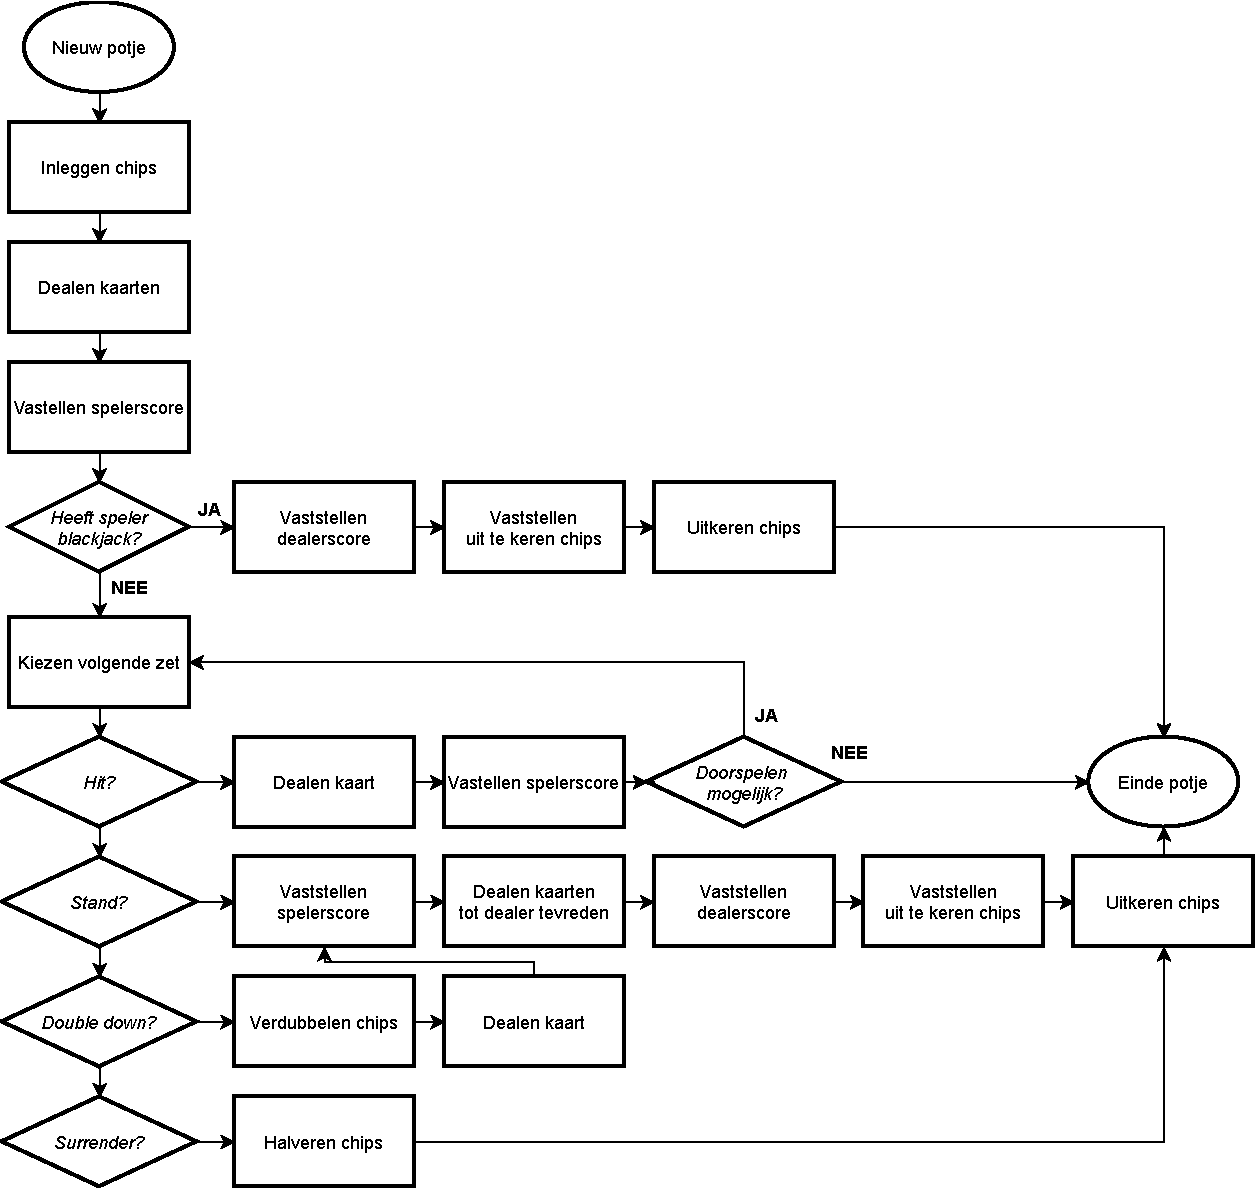
\includegraphics[width=\linewidth]{conceptual-flow-blackjack}
%     \caption{Conceptuele flowchart voor blackjack. 
%     Binnen een web-applicatie zal het er anders uitzien in verband met technische keuzes, efficiëntie en onderhoudbaarheid.}
%     \label{fig:conceptual-flow-blackjack}
% \end{figure}

\subsection*{Kaart- en handscore}
Per kaart wordt de score bepaald op basis van de rang (\textit{rank}) van de kaart:

\begin{itemize}
    \item \textbf{Getallen (2 - 10)}: de waarde die erop staat
    \item \textbf{Plaatjes (Jack, Queen, King)}: de waarde 10
    \item \textbf{Aas (Ace): 1 of 11}
\end{itemize}

De handscore wordt bepaald door deze scores bij elkaar op te tellen, 
zie Tabel \ref{table:handscores}.

\begin{table}[H]
    \centering
    \begin{tabularx}{0.4\textwidth}{|l|X|}
        \hline
        \textbf{Kaarten} & \textbf{Handscore} \\ \hline
        $\heartsuit 2, \clubsuit 3$ & 5 \\ \hline
        $\clubsuit 10, \diamondsuit 5, \heartsuit 3, \spadesuit2$ & 20 \\ \hline
        $\heartsuit 10, \clubsuit K$  & 20                 \\ \hline
        $\spadesuit A, \diamondsuit 4$ & 15 (of: 5)         \\ \hline
        $\clubsuit A, \diamondsuit K$ & 21 (of: 11)         \\ \hline
        $\clubsuit A, \heartsuit A$ & 12                 \\ \hline
    \end{tabularx}
    \caption{Voorbeelden van handscores.}
    \label{table:handscores}
    \centering
\end{table}

Merk op dat de aas ertoe leidt dat de speler kan kiezen om 
met de hogere aas-score uit te komen of te hopen op betere kaarten 
met de lagere aas-score. Als de hogere aas-score boven de 21 uitkomt,
hoeven we alleen nog maar te kijken naar de lagere aas-score.

\subsection*{Speltoestanden}
Er zijn een aantal toestanden waar het spel zich in kan bevinden:
\begin{itemize}
    \item \textit{Waiting}: het spel is aangemaakt, maar nog niet gestart (optioneel)
    \item \textit{Playing}: het spel is gestart en moves kunnen worden geselecteerd
    \item \textit{Bust}: speler heeft een handscore >21 en kan niet meer verder spelen
    \item \textit{Lost}: speler heeft een lagere eindscore dan de dealer
    \item \textit{Surrendered}: speler heeft het opgegeven
    \item \textit{Push}: speler heeft dezelfde handscore als de dealer of beiden hebben een handscore van 21 in de eerste beurt
    \item \textit{Blackjack}: speler heeft een handscore van 21 in de eerste beurt en de dealer niet
    \item \textit{Won}: speler heeft een hogere handscore dan de dealer of de dealer heeft >21
\end{itemize}

\subsection*{Uitbetaling}
Het uitbetalen van chips is gebaseerd op de eindtoestand (rond af naar hele chips).
Het spel eindigt alleen bij de volgende speltoestanden:

\begin{itemize}
    \item \textit{Bust}: speler krijgt niets terug
    \item \textit{Lost}: speler krijgt niets terug
    \item \textit{Surrendered}: speler krijgt $0.5\times$ zijn inleg terug
    \item \textit{Push}: speler krijgt $1\times$ zijn inleg terug
    \item \textit{Blackjack}: speler krijgt $1.5\times$ zijn inleg terug
    \item \textit{Won}: speler krijgt $2\times$ zijn inleg terug
\end{itemize}

\section*{Beoordeling}
Het gaat er bij dit vak om dat je een werkende en structureel goede back-end kan bouwen.
De snelste of kortste oplossing is voor deze cursus (en in de praktijk) niet altijd de beste oplossing!

\subsection*{Assessment}
We willen ook dat je je project kunt toelichten 
aan de hand van de voor de leerdoelen relevante behandelde stof.
Dit wordt getoetst aan de hand van een project met bijbehorend interview.

Het is verstandig om je project kort te presenteren met behulp van slides.
Sta daarbij alvast stil bij de theoretische onderbouwing.

\subsubsection*{Voorbeeldvragen}
Vragen die je kunt verwachten zijn gebaseerd op de leerdoelen van de cursus.
Je kan denken aan de volgende soort vragen:
\begin{itemize}
    \item Op welke manier heb je \textit{separation of concerns, loose coupling en high cohesion} bereikt?
    \item Wat houdt \textit{<object model element, design principle, design pattern>} in?
    \item Op welke manier heb je \textit{<design principle>} toegepast?
    \item Waarom zou je \textit{<object model element, design principle, design pattern, dependency injection>} gebruiken?
    \item Hoe heb je \textit{<design pattern>} in dit project uitgevoerd?
    \item Welk \textit{<design pattern>} zou je op \textit{<projectonderdeel>} kunnen toepassen?
    \item Op welke manier voldoe je aan \textit{<REST principe>}?
    \item Wat is de verantwoordelijkheid van \textit{<laag X>}?
\end{itemize}

\section*{Rubric}
Zie Canvas voor de rubric van het project. Heb je alle punten gehaald, dan haal je een 10.
Mocht je wat minder scoren op bepaalde onderdelen, dan wil dat niet zeggen dat je een onvoldoende hebt!
Hier kan je natuurlijk rekening mee houden wanneer je met een planning bezig gaat.